\chapter{INTRODUCTION}
\label{ch1}
Please note that all descriptions, references, figures and tables are for illustration purposes only.
All figures are taken from Megson's book on Aircraft Structures.

\section{MISSION REQUIREMENTS}
\label{s:ch1_intro}
Here you can include the mission requirements and motivation behind choosing the specific mission.
%
\section{CONFIGURATION CHOICE}
Briefly describe the configuration chosen and the rationale behind it.
If any of the configuaration choices are a direct consequence of the mission requirement mention that explicitly.
Following are the salient features of the configuration considered:
\begin{itemize}
\item High wing was chosen because .....
\item Delta wing was chosen for the following reasons: .
\item Airfoil was chosen to be XYZ because of bla bla bla.
\end{itemize}
 
\section{SUMMARY OF WORK DONE AS PART OF THE AERODYNAMIC DESIGN}
%
Here, a brief description (mandatory) should accompany data/ weight estimates and diagrams.
%
\subsection{Data Obtained from Literature Survey}
I guess title is self-explanatory.
Table \ref{tab:lit_survey} gives the details of existing aircrafts of similar configurations for which data were accessible.
I have deliberately made first column left justified, next 3 columns center justified and last columns right justified for demonstration purposes.
%
\begin{table}
\begin{center}
\caption{Details of the aircrafts available in literature.}
   \begin{tabular}{|l|c|c|c|r|r|r|}
   \hline
Brief description & Overall & Wing & Aspect &\multicolumn{3}{c|}{Weight fractions}  \\ \cline{5-7}
 & Weight (kg) & Span (m) & Ratio & Pay load & Power plant & Structural \\ \hline
 X1 & $a_1$ & $b_1$ & $c_1$ & $d_1$ & $e_1$ & $f_1$  \\ \hline
 X2 & $a_2$ & $b_2$ & $c_2$ & $d_2$ & $e_2$ & $f_2$  \\ \hline
 X3 & $a_3$ & $b_3$ & $c_3$ & $d_3$ & $e_3$ & $f_3$  \\ \hline
   \end{tabular}
\label{tab:lit_survey}
\end{center}
\end{table}
%
\subsection{First Weight Estimate}
I guess title is self-explanatory.
Next few sentences are included just to give you an idea as to how to include references and show you the difference between ``citep'' and ``citet'' commands.
\citet{Raymer_book} gives a description of procedure for weight estimation .
\citet{Joel_paper} is a review paper on design of UAVs.
Most UAVs below 1 $m$ wing span seem to use electric motors~\citep{random_book}.
%
\subsection{Second Weight Estimate}
I guess title is self-explanatory.
Let me just show you how to write an equation.
\begin{equation}
W = \frac{W_{payload}+W_{power plant}}{1-\overline{W}_{str}}
\end{equation}
%
\subsection{Third Weight Estimate}
I guess title is self-explanatory.
%
\subsection{Views of the Designed Airplane}
I guess title is self-explanatory.
Please ensure that the size of fonts used in the figure match the font size in the main body of the text.
If they dont, you can see how badly it looks (Figure \ref{fig:3view}) as compared to next two figures.
So, please dont have figures like this!!!!

Figure \ref{fig:3view} all three views of the aircraft with the detailed dimensions based on preliminary design.
%
\begin{figure}
\centering
\begin{minipage}{0.5\textwidth}
\begin{centering}
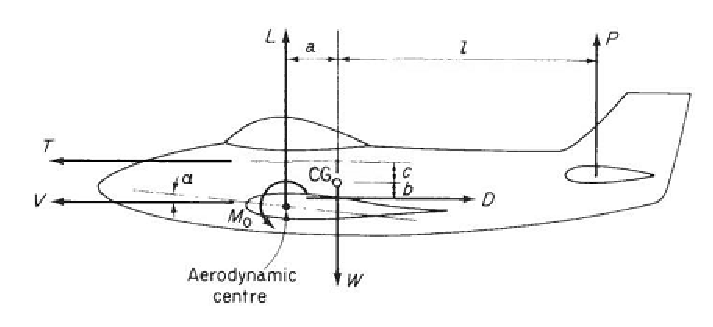
\includegraphics[width=\textwidth]{figures/side_view.eps}
\centerline{\small (a) Side View}
\end{centering}
\end{minipage}
\hspace{2mm}
\begin{minipage}{0.4\textwidth}
\begin{centering}
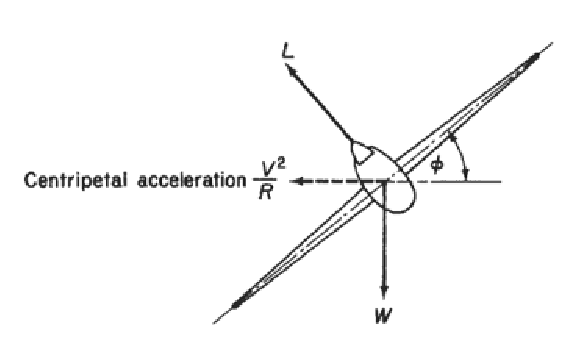
\includegraphics[width=\textwidth]{figures/front_view.eps}
\centerline{\small (b) Front View}
\end{centering}
\end{minipage}
%
\vspace{0.1in}
\begin{minipage}{0.5\textwidth}
\begin{centering}
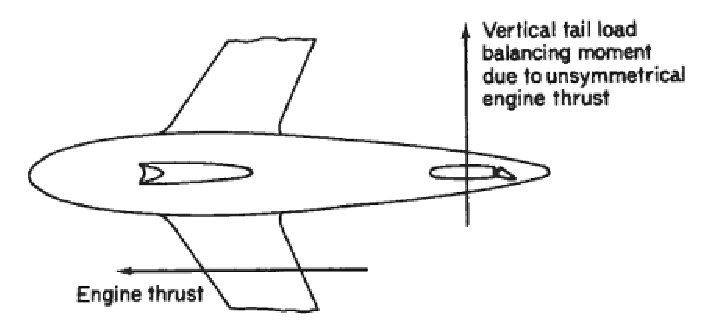
\includegraphics[width=\textwidth]{figures/top_view.eps}
\centerline{\small (c) Top View}
\end{centering}
\end{minipage}
\hspace{2mm}
\begin{minipage}{0.4\textwidth}
\begin{centering}
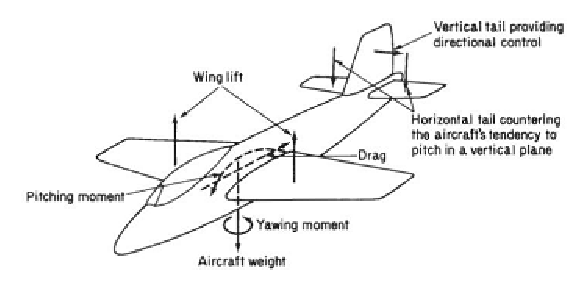
\includegraphics[width=\textwidth]{figures/3D.eps}
\centerline{\small (d) Side View}
\end{centering}
\end{minipage}
\caption{The 3D model and the meshed model of the proposed frame used for the modal analysis in ANSYS.}
\label{fig:3view}
\end{figure}
%
%
\subsection{V-n Diagram}
I guess title is self-explanatory.
Please ensure that the size of fonts used in the figure match the font size in the main body of the text.
Figure \ref{fig:V_n_diag} shows the envelope of the final V-n diagram for the chosen aircraft.
%
\begin{figure}
    \begin{center}
      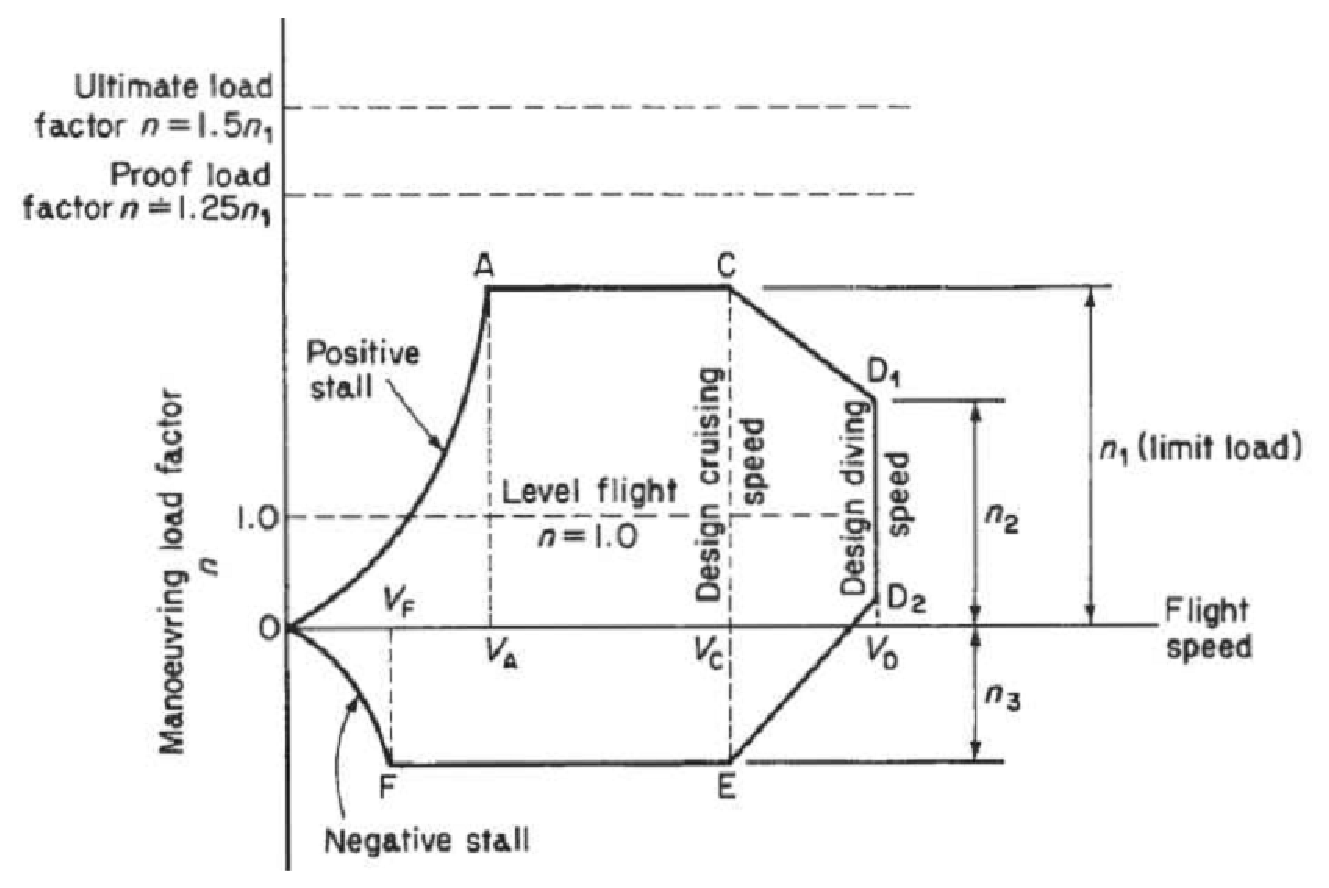
\includegraphics[width=6in]{figures/V_n_diag.eps}
\caption{Flight envelope: V-n diagram for the given airplane.}
       \label{fig:V_n_diag}
    \end{center}
\end{figure}
%

Figure \ref{fig:V_n_gust} shows the envelope of the final V-n diagram for the chosen aircraft including gust velocities of $\pm U_1$, $\pm U_2$ and $\pm U_3$.
%
\begin{figure}
    \begin{center}
      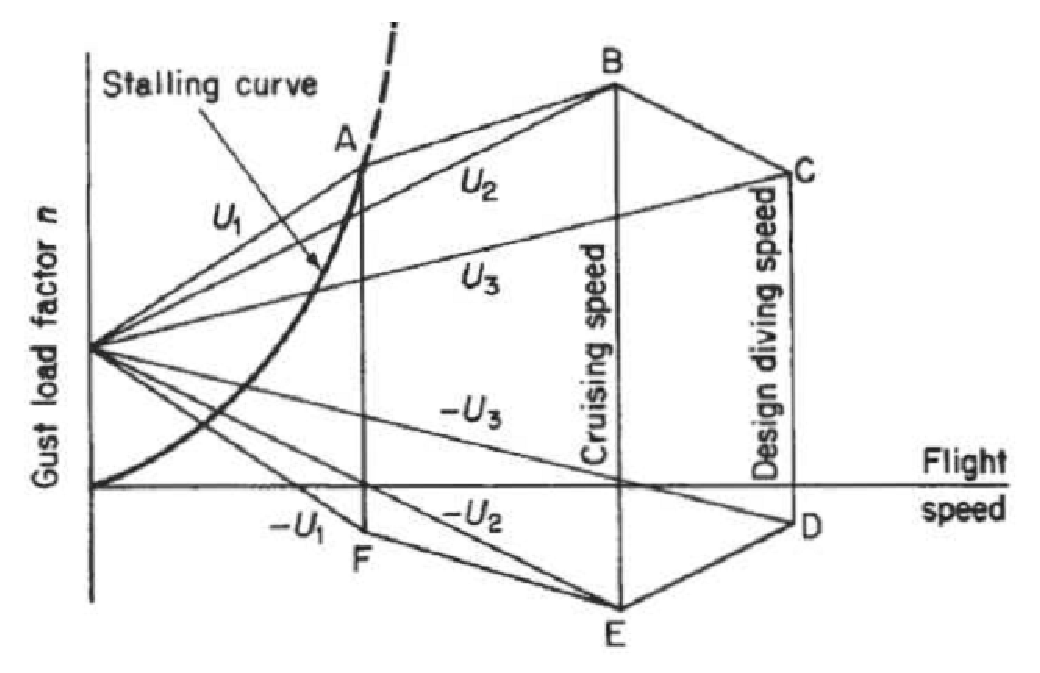
\includegraphics[width=4.5in]{figures/V_n_gust.eps}
     \caption{Gust envelope: V-n diagram for the given airplane for different gust velocities.}
       \label{fig:V_n_gust}
    \end{center}
\end{figure}
%
\section{Bill of Materials with suggested Vendors}
Table~\ref{tab:bill_materials} gives the details of the materials required for fabrication as well as suggested vendors and approximate cost ...

i have deliberately not put a vertical line between the first and second columns to demonstrate how to get or not to get horizontal lines separating the columns.
%
\begin{table}
\begin{center}
\caption{Bill of materials.}
   \begin{tabular}{|ll|l|}
   \hline
item description & Suggested vendor & Approximate cost \\ \hline
 X1 & $a_1$ & $b_1$  \\ \hline
 X2 & $a_2$ & $b_2$ \\ \hline
 X3 & $a_3$ & $b_3$ \\ \hline
   \end{tabular}
\label{tab:bill_materials}
\end{center}
\end{table}
%
%
